  \subsection{Emergency call}
The system detects an emergency, calls the NHS and send a text message to the contacts that are present in the emergency list.

\begin{table}[H]
	\centering
    
    \begin{tabular}{|p{3.5cm}|p{10.3cm}|}
    
    \hline
    \textbf{\large{Actors}}  			& NHS						     \\
    				 					
    \hline
    \textbf{\large{Goals}} 				& \ref{goal:sos1}                \\
    
    \hline
    \textbf{\large{Enter Condition}}	& The latest health data retrieved from the smart device exceed the critical parameters.		\\
    
    \hline
    \textbf{\large{Events Flow}}		& \begin{enumerate}[leftmargin=0.5cm]
                                          	\item The System creates a basic diagnosis based on the anomalous parameters. A text-to-speech algorithm generates the audio file from the diagnosis and the localization of the User.
                                            \item The System calls the \emph{NHS} emergency number and request the dispatching of an ambulance.
                                            \item The System sends a text message (SMS) to the contacts from the emergency list.
                                      \end{enumerate}
    										\\
    \hline
    \textbf{\large{Exit Condition}} 	& A call to the \emph{NHS} is performed by the System \\
    
    \hline
    \textbf{\large{Exception}} 			& The cellular credit is insufficient to deliver the text messages.\\
    								
    \hline
    
    \end{tabular}
	
\end{table}
\begin{figure}[H]
    \centering
    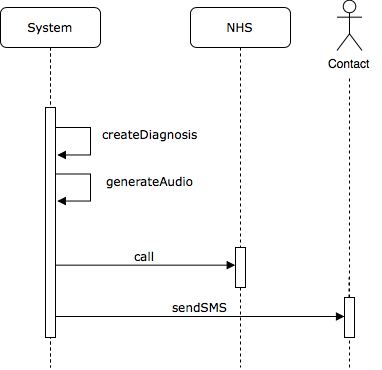
\includegraphics[scale=0.5]{rasdL/Pictures/emergency-sequence.png}
    \caption{Sequence diagram for the occurrence of an emergency status}
    
\end{figure}